% ── Base de Datos ────────────────────────────────────────────────────────────
\section{Base de Datos}

\subsection{Descripción general}

El diseño de la base de datos responde directamente a los requerimientos funcionales
identificados en el Sprint~1. Se optó por un modelo relacional implementado en
\textbf{PostgreSQL}, sistema gestor que ofrece soporte robusto para integridad
referencial, consultas complejas y transacciones seguras, características
indispensables para la gestión de trámites administrativos en una institución del
tamaño de la UNSAAC.

El modelo contempla once tablas que representan las entidades del dominio del problema:
especialidades, usuarios generales, usuarios administrativos, categorías, trámites,
requisitos, solicitudes, documentos, observaciones, seguimiento y notificaciones. Una
decisión de diseño central es la separación de los actores del sistema en dos tablas
independientes ---\texttt{usuario\_general} y \texttt{usuario\_admin}---, lo que
simplifica el control de acceso y refleja con claridad la distinción funcional entre
quienes realizan trámites y quienes los gestionan. Las relaciones entre las entidades
reproducen los flujos administrativos reales de la institución, desde la consulta del
catálogo del TUPA hasta la resolución y cierre de cada trámite.

\subsection{Diagrama Entidad-Relación}

A continuación se presenta el Diagrama Entidad-Relación (DER) del sistema, que ilustra
las entidades definidas, sus atributos principales y las relaciones entre ellas:

\begin{figure}[H]
  \centering
  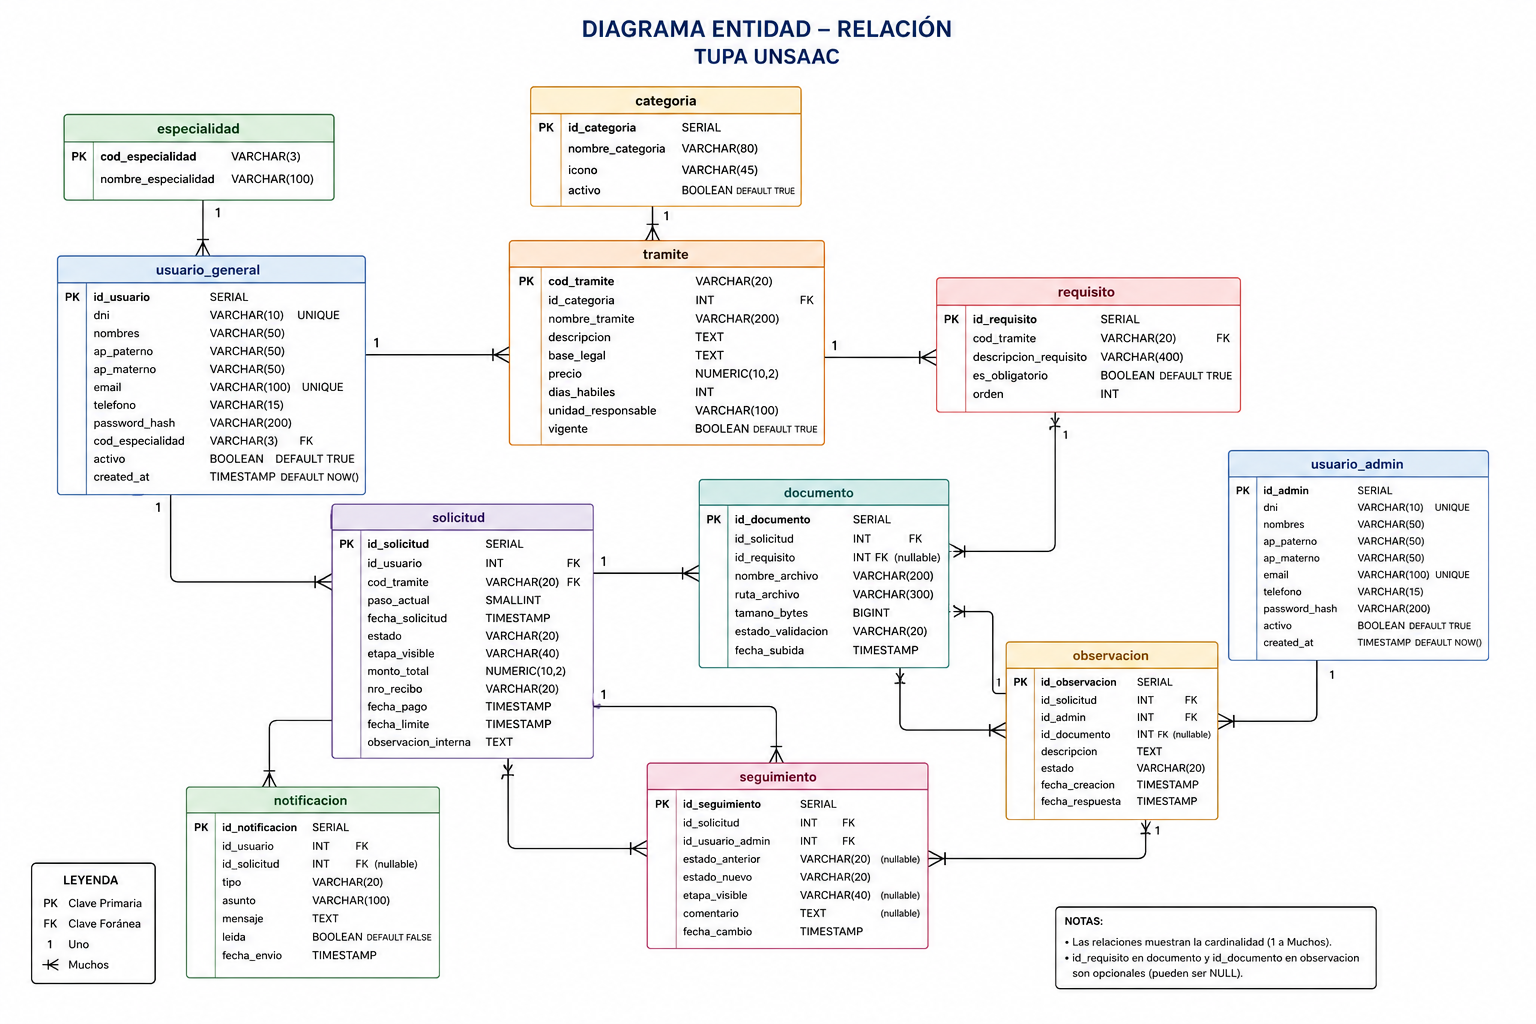
\includegraphics[width=0.9\textwidth]{images/DiagramaEntidadRelacion.png}
  \caption{Diagrama Entidad-Relación del sistema TUPA-UNSAAC}
  \label{fig:der-sistema}
\end{figure}

\subsection{Descripción de las entidades}

El modelo de datos está compuesto por las siguientes once entidades:

\begin{itemize}
  \item \textbf{Especialidad (\texttt{especialidad}):} catálogo de carreras y escuelas
        profesionales de la UNSAAC, identificadas por un código de tres caracteres
        (\texttt{cod\_especialidad}). Permite vincular a cada usuario general con su
        programa académico correspondiente.

  \item \textbf{Usuario General (\texttt{usuario\_general}):} almacena la información
        de los usuarios que realizan trámites ante la universidad. Registra DNI, nombres,
        apellidos, correo electrónico, teléfono, credenciales de acceso y la especialidad
        académica a la que pertenecen. Estos usuarios pueden consultar el catálogo del
        TUPA, iniciar solicitudes a través del wizard de seis pasos, cargar documentos y
        dar seguimiento al estado de sus trámites.

  \item \textbf{Usuario Admin (\texttt{usuario\_admin}):} representa al personal
        administrativo del sistema. Registra los mismos datos personales y de
        autenticación que el usuario general, pero sin vinculación a una especialidad
        académica. Los administradores revisan solicitudes, validan documentos, emiten
        observaciones, cambian estados de trámites y consultan los indicadores de gestión
        del panel administrativo.

  \item \textbf{Categoría (\texttt{categoria}):} agrupa los trámites del TUPA en
        clasificaciones temáticas (Académicos, Facultad, Investigación, Bienestar,
        entre otros) para facilitar la navegación y filtrado en el catálogo público.
        Incluye un atributo de ícono para su representación visual en la interfaz.

  \item \textbf{Trámite (\texttt{tramite}):} tabla central del catálogo público,
        representa cada uno de los procedimientos contemplados en el TUPA vigente.
        Registra el código del trámite, su nombre, descripción, base legal que lo
        sustenta, precio, plazo de atención en días hábiles, unidad orgánica responsable
        y estado de vigencia. Cada trámite pertenece a una categoría.

  \item \textbf{Requisito (\texttt{requisito}):} documenta las condiciones y documentos
        necesarios para iniciar cada trámite. Cada requisito está vinculado a un trámite
        específico e incluye su descripción, carácter obligatorio u opcional y un orden
        de presentación. Se muestra tanto en el catálogo público como en el paso~3 del
        wizard de solicitud.

  \item \textbf{Solicitud (\texttt{solicitud}):} entidad central del ciclo de vida de
        un trámite, registra cada procedimiento iniciado por un usuario general. Gestiona
        el estado interno del proceso (\texttt{BORRADOR}, \texttt{SOLICITADO},
        \texttt{EN~PROCESO}, \texttt{PAGADO}, \texttt{SUBSANACION}, \texttt{COMPLETADO}
        o \texttt{ANULADO}), la etapa visible en la línea de tiempo, el paso actual del
        wizard (1~a~6, con restricción \texttt{CHECK}), las fechas relevantes, el monto
        total, el número de recibo y los datos de pago asociados.

  \item \textbf{Documento (\texttt{documento}):} almacena las referencias a los archivos
        digitales que el usuario carga durante el paso~3 del wizard. Cada documento se
        vincula a la solicitud correspondiente y al requisito específico que cubre,
        registrando el nombre del archivo, su ruta en el servidor, tamaño en bytes y
        estado de validación (\texttt{PENDIENTE}, \texttt{APROBADO} o
        \texttt{RECHAZADO}).

  \item \textbf{Observación (\texttt{observacion}):} registra las incidencias señaladas
        por un administrador sobre documentos específicos de una solicitud. Cuando un
        documento presenta un problema, el administrador emite una observación con la
        descripción del defecto detectado, vinculada al documento en cuestión. El estado
        de la solicitud cambia automáticamente a \texttt{SUBSANACION} y se genera una
        notificación al usuario para que corrija y vuelva a cargar la documentación.
        La observación puede pasar por los estados \texttt{PENDIENTE},
        \texttt{SUBSANADO} y \texttt{CERRADO}.

  \item \textbf{Seguimiento (\texttt{seguimiento}):} log de auditoría que registra de
        forma cronológica todos los cambios de estado de una solicitud. Cada entrada
        almacena el estado anterior, el estado nuevo, la etapa visible correspondiente,
        un comentario opcional y la referencia al administrador que ejecutó el cambio.
        Esta tabla alimenta la línea de tiempo visual del módulo de seguimiento del
        usuario.

  \item \textbf{Notificación (\texttt{notificacion}):} registra las alertas enviadas
        automáticamente a los usuarios generales ante eventos relevantes: cambios de
        estado (\texttt{ESTADO}), observaciones emitidas (\texttt{OBSERVACION}),
        verificación de pagos (\texttt{PAGO}) o proximidad de vencimiento
        (\texttt{VENCIMIENTO}). Cada notificación incluye asunto, mensaje, indicador
        de lectura y la solicitud asociada.
\end{itemize}

\subsection{Consideraciones de diseño}

El modelo adopta las siguientes decisiones de diseño relevantes:

\begin{itemize}
  \item La separación de usuarios en dos tablas independientes
        ---\texttt{usuario\_general} y \texttt{usuario\_admin}--- responde a la
        distinción funcional clara entre los actores del sistema: los usuarios generales
        inician y dan seguimiento a trámites, mientras que los administradores gestionan,
        validan y resuelven solicitudes. Esta separación simplifica las consultas, evita
        columnas nulas innecesarias (como \texttt{cod\_especialidad} para
        administradores) y facilita la implementación de políticas de acceso
        diferenciadas en el backend.

  \item Los documentos adjuntos se almacenan como referencias a rutas de archivos en el
        servidor (atributo \texttt{ruta\_archivo}), no como datos binarios en la base de
        datos, lo que optimiza el rendimiento de las consultas y facilita la gestión
        independiente del almacenamiento.

  \item La tabla \texttt{seguimiento} se mantiene como entidad independiente para
        garantizar la trazabilidad completa del ciclo de vida de cada trámite sin
        modificar los registros originales de la solicitud, respetando principios básicos
        de auditoría de datos y permitiendo reconstruir la línea de tiempo completa de
        cualquier procedimiento.

  \item El sistema distingue entre el \textbf{estado interno} de una solicitud (utilizado
        por la lógica de negocio: \texttt{BORRADOR}, \texttt{SOLICITADO}, etc.) y la
        \textbf{etapa visible} (texto mostrado al usuario en la línea de tiempo:
        \emph{Recibido}, \emph{Evaluación técnica}, \emph{Pago verificado}, etc.), lo
        que permite adaptar la comunicación al usuario sin alterar la máquina de estados
        del proceso administrativo.

  \item Se definieron índices sobre las columnas de consulta más frecuente ---DNI, email,
        estado de solicitud, fecha, relaciones foráneas y notificaciones no leídas---
        para optimizar el rendimiento de las operaciones de búsqueda y filtrado en los
        módulos de catálogo, seguimiento y panel administrativo.
\end{itemize}

\subsection{Relaciones entre entidades}

Las relaciones principales del modelo se resumen a continuación:

\begin{itemize}
  \item \texttt{especialidad} $\rightarrow$ \texttt{usuario\_general}: una especialidad
        puede tener múltiples usuarios generales asociados.
  \item \texttt{categoria} $\rightarrow$ \texttt{tramite}: cada categoría agrupa
        múltiples trámites del catálogo.
  \item \texttt{tramite} $\rightarrow$ \texttt{requisito}: cada trámite define uno o
        más requisitos documentales.
  \item \texttt{usuario\_general} y \texttt{tramite} $\rightarrow$ \texttt{solicitud}:
        cada solicitud vincula a un usuario general con un trámite específico.
  \item \texttt{solicitud} y \texttt{requisito} $\rightarrow$ \texttt{documento}: cada
        documento cargado se asocia a una solicitud y al requisito que cubre.
  \item \texttt{solicitud} y \texttt{usuario\_admin} $\rightarrow$
        \texttt{observacion}: las observaciones son emitidas por un administrador sobre
        una solicitud, vinculadas opcionalmente a un documento específico.
  \item \texttt{solicitud} y \texttt{usuario\_admin} $\rightarrow$
        \texttt{seguimiento}: cada cambio de estado es registrado por un administrador
        como entrada de auditoría.
  \item \texttt{usuario\_general} y \texttt{solicitud} $\rightarrow$
        \texttt{notificacion}: las notificaciones se dirigen a un usuario general y se
        asocian a una solicitud.
\end{itemize}

\begin{figure}[H]
  \centering
  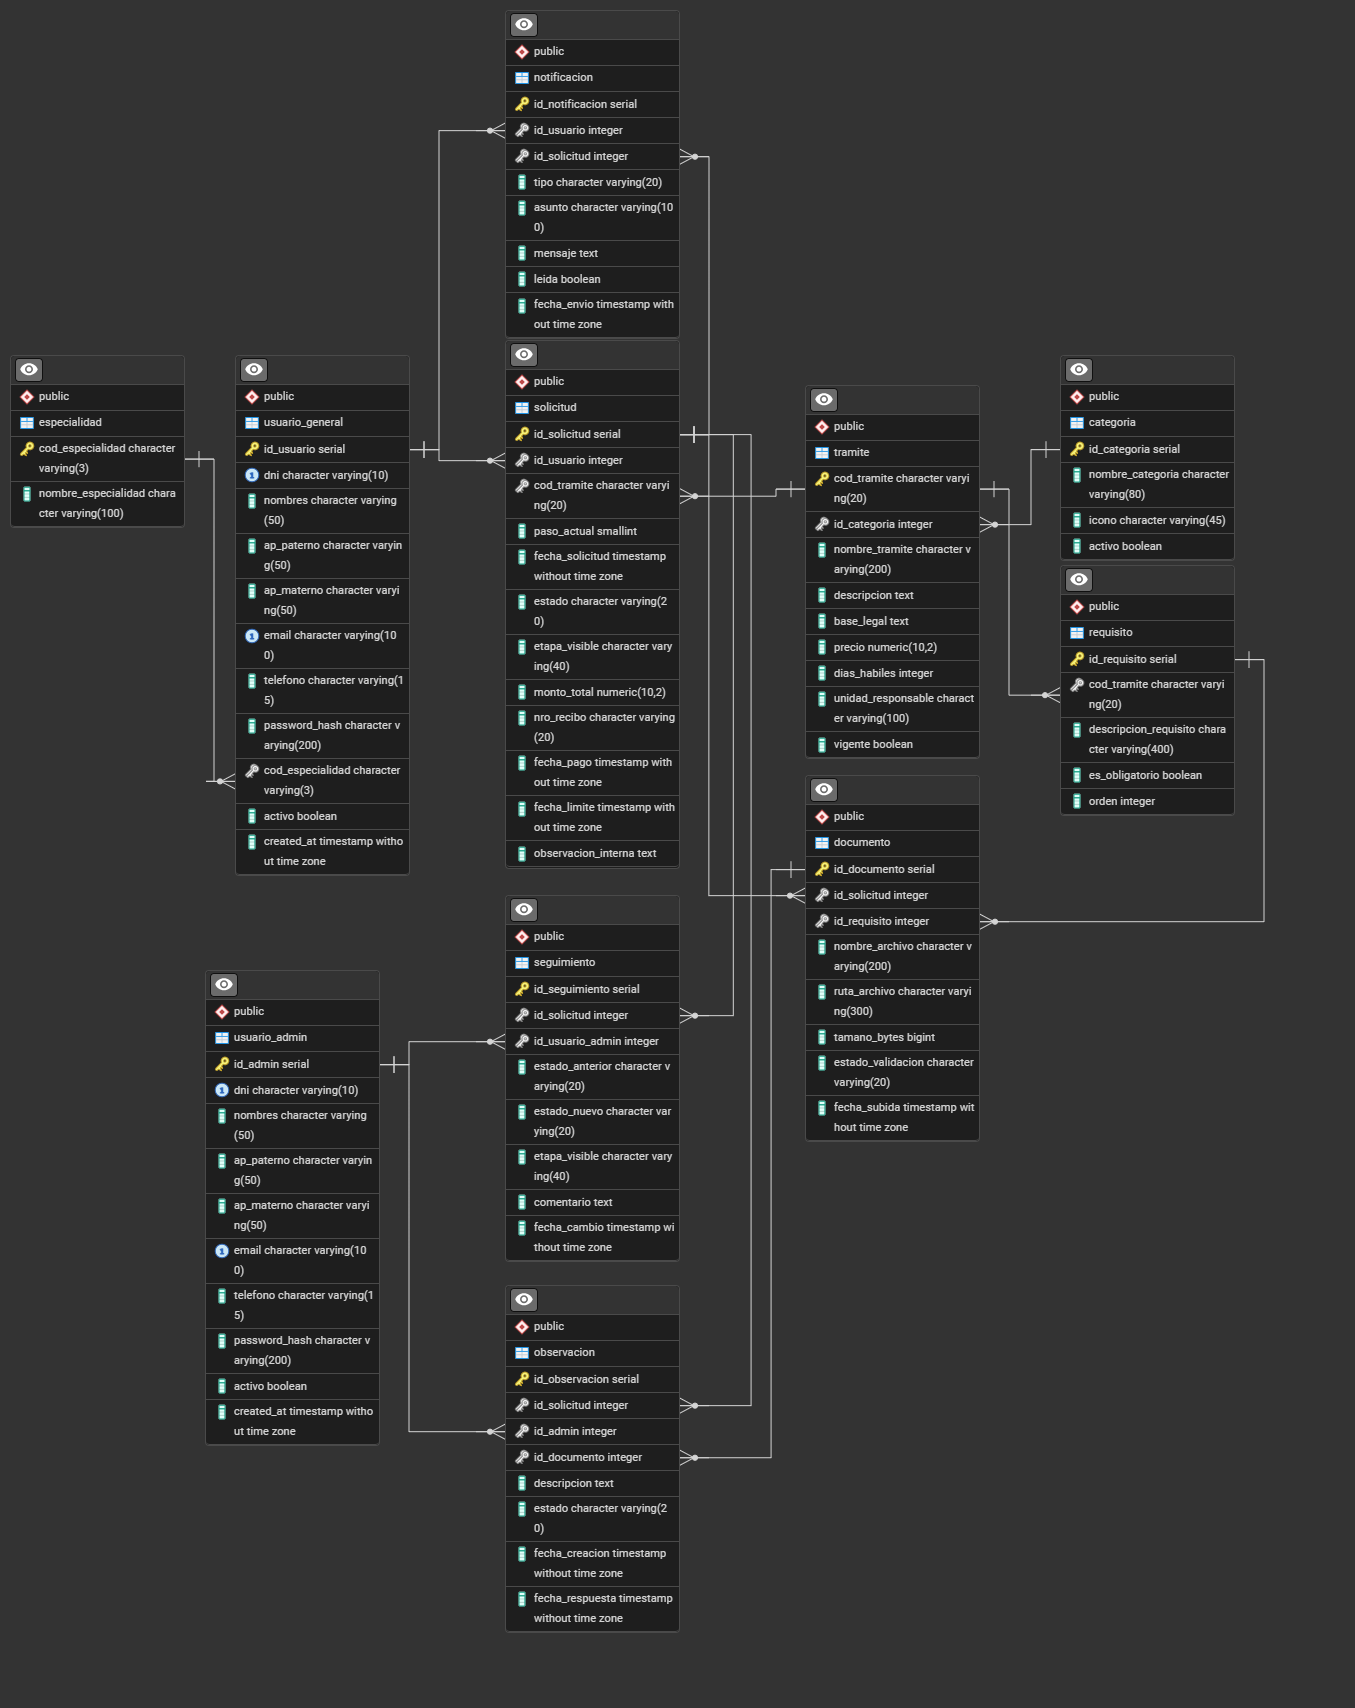
\includegraphics[width=0.9\textwidth]{images/BDDDiagram.png}
  \caption{Modelo relacional de la base de datos --- diagrama físico}
  \label{fig:modelo-relacional}
\end{figure}
